So far we have introduced a type system and process calculus for writing and checking runtime that conforms to the import mechanism for polynomial runtime.
In this section, we show that NomosUC can realize any arbitrary ITM configuration, as possible in UC, and that we can easily encode the set of fundamental proofs and lemmas of the framework and a generic composition operator.
The main challenges we overcome in realizing arbitrary ITM systems is grappling with the parent-child relationship between processes (and the provider-client reationship in channels) that prevents cyclical topologies in the normal case. 
We introduce a simple construction called \emph{providerless channels} which relies on shared session types and uses our virtual token construction. 
Second we discuss how the dummy lemma, a composition operator, and the composition theorem can be realized by the introduction of \emph{providerless channels}.

\subsection{Expressivity}
The first thing we need to show, to argue that NomosUC can realize the full expressivity of UC. 
The ITM computational model is extremeley flexible to capture as universal a setting as possible.
Channels in NomosUC are linear, created by some process known as the provider, and impose a strict parent-child relationship. 
Unlike the ITM model, this model prohibits cyclical topologies: a process $A$ offers a channel to $C$, which offers a channel to $B$, which offers a channel to $A$ can not be realize by NomosUC.

To enable arbitrary communication between two processes without forcing a parent-child relationship, we introduce
the concept of \emph{providerless channels} using \emph{communicator processes} that rely on recently introduced shared session types~\cite{balzer2017manifest}.
Communicators act as a buffer between two processes allowing them to exchange messages via the communicator.
Communicators also break the parent-child relationship by offering a \emph{shared channel that can have multiple clients}
(unlike linear channels that can have only one client) that is then used by both the sender and receiver processes.

The communicator has the following polymorphic type:
%\begin{center}
\vspace{-1mm}
{\centering
\parbox{0cm}{
\begin{tabbing}
$\m{comm[\tau]\{n\}} = \up \echoice{$\=$ \textcolor{red}{\getpot^n} \mb{push}: \m{\tau} \arrow \m \down \m{comm[\tau]},$\\
\>$\textcolor{red}{\getpot^0} \mb{poll}: \ichoice{$\=$\textcolor{red}{\paypot^{n-1}} \mb{yes}: \m{\tau} \;\product \down \m{comm[\tau]},$\\
\>\>$\textcolor{red}{\paypot^0} \mb{no}: \; \down \m{comm[\tau]}}}$
\end{tabbing}}
%\end{center}
\par}

The communicator type uses the type constructions $\up$ and $\down$ to indicate that 
access to the channel must be \emph{acquired} and eventually \emph{released}, respectively.
The acquire-release paradigm, along with the write token, is necessary for shared session types to prevent non-determinism.
Communicators are written to by a sender that acquires the channel and $\mb{push}$es a functionally 
typed message along with some amount of import indicated as a parameter. A receiver acquires the 
channels and asks the communicator for new messages with $\mb{poll}$ if there is a message it is returned with some import
otherwise the channels takes the $\mb{no}$ branch.
We provide the full typing rule of shared session types in Appendix~\ref{app:typing_rules}.
\begin{figure}
	\begin{subfigure}{0.5\textwidth}
	\begin{center}
	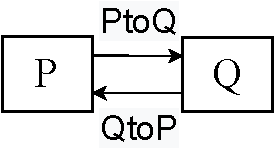
\includegraphics[scale=0.5]{figures/p_and_q.pdf}
	\caption{Goal: $P$, $Q$ connected by channels labeled with their types.}
	\label{fig:pandq}
	\end{center}
	\vspace{0.1em}
	\end{subfigure}
	\begin{subfigure}{0.5\textwidth}
	\begin{center}
	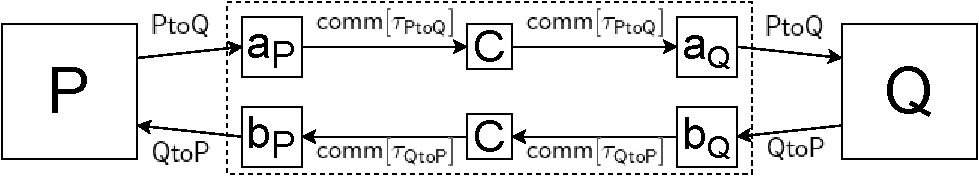
\includegraphics[scale=0.4]{figures/newPandQ.pdf}
	\caption{Internal implementation of channels using communication\\wrapper
	with channels labeled with their session types.}
	\label{fig:newpandq}
	\end{center}
	\end{subfigure}
	\caption{Two ITM configurations. One possible with ITMs (top) and one realized in NomosUC (bottom). Arrows indicate direction of messages
	and labels indicate types.}
	\vspace{-1em}
\end{figure}


All processing communication through communicators are relgeated to using the same session type. 
Even if we can realize cylcical topologies, we lose protocol/functionality-specific session types.
Providerless channels connecting some processes $P$ and $Q$ consist of shared channels and dummy processes that speak to $P$ (and $Q$) with the session type they expect and send messages to the communicator. 
In Figure~\ref{fig:newpandq} we show an illustration of a providerless channel between the two processes. 
Here, the processes intend to communicate through two unidiretional channels (a cycle) with the session types \m{PtoQ} and \m{QtoP}.
The dummy processes $a_P$ and $a_Q$ offer the channels to $P$ with the session requisite session types.
On message from $P$, $a_P$ case matches on the label in the session type and sends a functionally typed message of type $\tau_\m{PtoQ}$ to the communicator. 
Similarly, when $a_Q$ receives a message from the communicator, it case matches on the message in the buffered message and sends the corresponding label on the linear channel, with type \m{PtoQ}, to $Q$. 
The dummy processes consist only of case matches and, therefore, given some mapping between the labels of \m{PtoQ} and $\tau_\m{PtoQ}$, $a_P$ is trivially generated. 

The advantage of this construction is that it is simple, the dummy processes are trivial, the type system can enforce message ordering (as well as the $\paypot{R}$ and $\getpot{R}$ type constructors), and a system of processes can be arbitrarily connected. 
For example, if \Fdb from the previous section is connected to a party with a providerless channel, 
$\m{db}[k][v]$ remains the same and $\tau_\m{db[k][v]} =$ \inline{Store of PID k v |} \inline{OK of PID |} \inline{Get of PID k |} \inline{Yes of v | No}. 

Intuitively, this construction lets us show a bisimulation between NomosUC terms and ITMs.
We conclude in Appendix~\ref{app:itm} that we can realize any NomosUC configuration as a sytem of ITMS and that any ITM system can be realized as a Nomos UC configuration (NomosUC $C' \Leftrightarrow$ ITMs $M'$).
\todo{maybe we should have a few lines here, or a paragraph, making clear that providereless channels are generated at compile-time given the session types and $\tau$ functional message types by the programmer.}

\paragraph*{\textbf{Dynamic Parties}}
A major limitation of prior UC formalisms is supporting a subset of UC where only a static number of parties is allowed.
Providerless channels and sandboxing allow NomosUC to support dynamic party creation, at runtime, by \Z and \A.
Rather than create new linear channels on the fly and connect new parties to \Z and \A, we create a \emph{party wrapper}: a single endpoint that communicates with \Z, \A and the functionality and manages the creation and communication or protocol parties.
We reuse the labelling from Figure~\ref{fig:newpandq}.
The \partywrapper communicates with generic session types where messages are multiplexed by \m{PID}.
For example, communication from \partywrapper to \Fdb is mediated by a providerless channel where the session type is
\begin{tabbing}
	$\mi{type} \; \m{P2F[\tau]\{n\}} = \ichoice{\textcolor{red}{\paypot{n}} \; \mb{p2f}: \m{PID} \arrow \m{\tau} \arrow \m{P2F[\tau]\{n\}}}$
\end{tabbing}
where $\tau =$ \inline{Store $\tg{ of }$ k v | Get $\tg{ of }$ k} and $n = 1$, and the opposite direction is intuitive. 

New parties are spawned the first time they're sent a message.
First the \partywrapper creates providerless channels to communicate with them, and then it passes them as parameters to the new protocol party--all with a virtual token type.
When a message arrives, the \partywrapper chooses the correct channel from a list, withdraws the necessary virtual tokens, and forwards the message.
It waits on all of the outgoing channels of that party for a new message and forwards it externally.
An example of message routing that the \partywrapper does is given in Appendix~\ref{app:arbparties}.
\todo{if we have space we should put that example here.}

\subsection{The UC Experiment}
%In this section we highlight how \m{execUC} is encoded in NomosUC.
%Recall from Section~\ref{sec:basic} that linear session types impose constraints on what forms of communication can be captured, and pose challenges to supporting 
%a dynamic number of protocol parties, or functionalities, at runtime. 
%We detail how our encoding realizes dynamic parties through the use of virtual tokens in our \partywrapper,
%and validate our encoding by realizing a few critical results from the UC literature: the Dummy Lemma, a composition operator, and a multisession operator. 
%These three results allow us to ultimately conclude that NomosUC realizes full UC composition.
%We also run through a case of a coin-flip protocol, composed with the cryptographic commitment, in the Appendix. 

% \subsection{The UC Experiment}
The definition of \m{execUC} is straightforward owing to our mechanism of providerless channels. 
\m{execUC} is aways parameterized by at least one virtual token type to allow for sandboxing (specifically for the \partywrapper)
and message type parameters for the protocol in question. 
It also takes in a security parameter $k$ and a random bit string $r$ that is used as a source of
randomness for all future processes.
\m{execUC} offers the following type:
\begin{center}
\vspace{-2mm}
\parbox{0cm}{
\begin{tabbing} 
 $\m{execout}[\K][a]\{n\} = \echoice{ \textcolor{red}{\getpot^{\{n : \K\}}}\mb{exec}: $\=$ \m{Bit} \product 1}$ 
 \end{tabbing}}
\vspace{-2mm}
\end{center}
The type is parameterized by the real token type $\K$, message type $a$ and the import quantity $n$.
The type $\m{execout}[a]$ accepts $n$ import tokens and an $\mb{exec}$ message, and returns an output \m{Bit} as the result from \Z. 
With the help of the super-additive conversion function, the NomosUC type system ensures
that the runtime bound of \m{execUC} is $poly(k)$ as long as the number of tokens $n \in poly(k)$.

\m{execUC} only spawns processes already wrapped according to the providerless channel specification in Section~\ref{sec:basic}.
Therefore, it only has to spawn the part of the channel that connects wrapped processes.
We make this separation because the wrapped processes code is autogenerated given a specification of the session type and functional
type associated with the process.

%All main processes in NomosUC are wrapped according to the providerless channel specification in Section~\ref{sec:basic}. 
%Therefore, \m{execUC} creates only the part of the providerless channel (e.g. $\m{PtoQ}$ channel from Figure~\ref{fig:newpandq})
%and passes them as input to the communicator wrappers.
%The wrapper creates the intermediate processes and the shared session types providing the linear channel to \m{execUC}.
%For example \Z and \A are connected by the following channels:
%\begin{lstlisting}[basicstyle=\footnotesize\BeraMonottFamily, mathescape]
%$\$$ztoa $\leftarrow$ channel_init[$\tp{G}$][$\tp{z2a}$]{$\tp{z2an}$}
%$\$$atoz $\leftarrow$ channel_init[$\tp{G}$][$\tp{a2z}$]{$\tp{a2zn}$}
%$\tg{...}$
%$\$$z <- env[G] k rng $\$$ztop $\$$ptoz $\$$ztoa $\$$atoz ;
%\end{lstlisting}

Once channels are created, the environment \Z is the first process to be spawned.
As it's type \m{EtoZ} indicates below, it determines the main parameters of the experiment: the session id (\m{SID}) according to a user-defined type, and 
it determines the set of corrupt parties. 
\Z starts execution given some import $n$ by \m{execUC}.
These are given by \m{execUC} to the rest of the processes it spawns. 
\begin{center}
\vspace{-2mm}
\parbox{0cm}{
\begin{tabbing}
 $\m{EtoZ}[a]$ = $\m{SID}[a] \arrow [\m{PID}] \arrow \echoice{\textcolor{red}{\getpot^n} \mb{start}: \m{Bit} \arrow 1}$
 \end{tabbing}}
\vspace{-2mm}
\end{center}
%The type dictates that \Z sends the SID and the corruption list to \m{execUC},
%and \m{execUC} passes them as parameters to \F, \A and the \partywrapper.  
%\Z starts on input \mb{start} with $n$ tokens. 
Finally, the output bit, \Z's guess of which world it is in, forms the basis of the definition of indistinguishability.

\paragraph*{\textbf{The \partywrapper}}
We create the \partywrapper to handle process spawn, channel creation and connection to the rest of the experiment.
Instead of parties directly communicating with \F and \Z through providerless channels, the \partywrapper runs them virtually and presents a ``real'' view to them.
Virtual tokens enable us to simulate the protocol parties and satisfy the import their session types require while sandboxing them. 
The \partywrapper, in turn, is connected by a channel to each of \F, \Z, and \A and routes communication to/from the appropriate protocol party. 
Its design forces the wrapper around \F to do the same. It must de-multiplex inputs from the \partywrapper and react similarly to messages fro newly created parties. 

\paragraph*{\textbf{Emulation}}
The central security definition in UC is indistinguishability between the real and ideal world experiments.
It is defined in terms of the ensemble of distributions created by the output bits from the partial term
$(\m{execUC}\ \pi\ \F)$ over all possible random inputs and security parameters. 
We say that two worlds are indistinguishable if $\forall \A\ \exists \Sim\ \forall Z$
the \emph{statistical difference} in ensembles from the two worlds is negligible in $k$ (see
Definition~\ref{def:emulation} below).

\begin{definition}[Emulation]\label{def:emulation}
If two protocols $(\pi, \F_1)$ and $(\phi, \F_2)$, which we refer to only
by \PI and $\phi$, emulated each other, then $\forall \A$ of type $\Delta_3'$ well-matched with \PI, there must $\exists \Sim$ of the same type,  well-matched with $\phi$, s.t. $\forall \Z$ : $\msf{execUC}(\pi, \F_1, \Z, \A)$ $\approx$ $\msf{execUC}(\phi, \F_2, \Z, \Sim)$:

\begin{mathpar}
	\footnotesize
	\inferrule*[right=emulate]
	{
		\F_1 : \Delta_{\F_1}', \F_2 : \Delta_{\F_2}' \semi
		\Delta_{\F_1}' \vdash \pi : \Delta_1' \semi \Delta_{\F_2}' \vdash \phi : \Delta_2' \semi \\
		\forall \A \ . \ \Delta_4, \Delta_1' \vdash \A :: \Delta_3', \matched{\A}{\pi}, \matched{\A}{\F_1} \\
		\Rightarrow \exists \Sim_\A \ . \ (\Delta_3, \Delta_2' \vdash \Sim_\A :: \Delta_3'), \matched{\Sim_\A}{\phi}, \matched{\Sim_\A}{\F_2} \semi \\
		\forall \Z \ . \ \matched{\Z}{\pi}, \matched{\Z}{\phi} \Rightarrow \\
		\msf{execUC} \ \pi\ \F_1\ \Z\ \A \sim \msf{execUC} \ \phi\ \F_2\ \Z\ \Sim_\A
	}
	{
		% EMULATION DEFINITION
		\lambda \A \, . \, \Sim_\A \vdash (\pi, \F_1) \sim (\phi, \F_2)
	}
\end{mathpar}
\end{definition}
The notation $e \leftrightarrow e'$ is used to denote two \emph{well-matched} process terms meaning
that they have the \emph{same type on all the channels} used and provided.

% \paragraph*{\textbf{Dummy Lemma}}
\begin{theorem}[Dummy Lemma]\label{thm:dummythicclemma}
If \ $\exists \DS$ s.t. $ \DA, \DS \vdash \F_2 \xrightarrow{\pi} \F_1$ then $\forall \A \ \exists \Sim_\A$ s.t. $\Sim_{\A} \vdash  \F_2 \xrightarrow{\pi} \F_1)$ 
\end{theorem}
An important validation of our approach is the Dummy Lemma which shows that a simulator \DS for the dummy adversary, suffices to prove emulation. 
The proof of the Lemma is in the form of a constructor for a simulator for any arbitrary real world \A (in Appendix~\ref{sec:dummy}).
The simplicity of the simulator construction and the resulting simulation proof highlights the
simplicity and expressiveness that our token hierarchy and sandboxing afford. 

\paragraph*{\textbf{Single Composition}}
Recalling Theorem~\ref{thm:singlecomp}, composition allows replacement of a single ideal functionality $\F_2$ with a protocol $\pi$ that realizes it in the $\F_1$-hybrid world. 
A protocol party $\rho_i$ that gives input to $\F_2$ instead gives input to party $\pi_i$ through a providerless channel in the \partywrapper. 
Like \m{execUC} (full code in the Appendix), the operator connects wrapped processes with providerless channels as shown below. 
%%\begin{lstlisting}[basicstyle=\footnotesize\BeraMonottFamily, mathescape, frame=single]
%%$\nproc$ compose[$\tg{...}$][rho2f,f2rho]{rho2fn,f2rhon}
%%  $\tg{(* args *)}$ |- ($\$$ch: 1) = 
%%#rho2pi $\leftarrow$ channel_init[G][rho2f]{rho2fn} ;
%%#pi2rho $\leftarrow$ channel_init[G][f2rho]{f2rhon} ;
%%  
%%$\$$r $\leftarrow$ rho $\leftarrow$ k rng sid pid #z2p #p2z #rho2pi #pi2rho; 
%%$\$$p $\leftarrow$ pi $\leftarrow$ k rng sid pid #rho2pi #pi2rho #p2f #f2p;
%%\end{lstlisting}

\begin{lstlisting}[basicstyle=\footnotesize\BeraMonottFamily, mathescape, frame=single]
$\nproc$ compose[K,K1,s][z2rho,rho2z][pi2f,f2pi]$\tg{...}$
  (k: Int), (rng: [Bit]), (sid: SID[s]), (pid: PID),
  (#z2p: comm[K][z2rho]{z2rhon}), $\tg{...}$ 
  (#p2f: comm[K][pi2f]{pi2fn}) $\tg{...}$
    $\vdash$ ($\$$ch: 1) =
{
  #rhop2f $\leftarrow$ channel_init[K][rho2f]{rho2fn} ;
  #piz2p $\leftarrow$ wrap_z2p[K][rho2f]{rho2fn} $\leftarrow$ #rhop2f ;
  #piz2p $\leftarrow$ channel_init[K][rho2f]{rho2fn} ;
  #rhof2p $\leftarrow$ wrap_p2z[K][rho2f]{rho2fm $\leftarrow$ #piz2p ;

  $\leftarrow$ gen_wrapper_rho[K1] $\leftarrow$ 
    k rng sid pid #z2p #p2z #rho2pi #pi2rho ;
  $\leftarrow$ gen_wrapper_pi[K1] $\leftarrow$ 
    k rng sid pid #rho2pi #pi2rho #p2f #f2p ; 
}
\end{lstlisting}
As indicated the operator deals with the wrapped versions of $\rho$ and $\pi$, and its parametric type ensures that any two protocols, especially multisession versions of them ($!\pi$), can be composed together.
The two protocol parties are connected in the obvious way with output from $\rho$ wrapped into the a type \inline{Z2P} to making it look like input from \Z to $\pi$.

%The operator interacts with the wrapped versions of the constituent protocols $\rho$ and $\pi$, and its parametric type ensures that even multisession versions of a protocol $\pi$ can be composed with $\rho$.
%It creates channels between the two parties and wraps the message sent from $\rho$ to appear as input from \Z to $\pi$. 
%
%In the next section we talk briefly about building a zero-knowledge UC experient by applying the multisession extension of $!\Fcom$ used throughout this work.
%We talk about it at a high-level and relegate a more detailed specification of the protocol in the appendix.

Proving UC security under composition requires creating a simulator for $\rho \circ \pi$ that realizes $\F_3$. 
This is done by connecting the two simulators, \SIM{\pi} and \SIM{\rho}, in the same way as the Dummy Lemma: sandboxed \SIM{\pi} receives input from \Z, gives output to \SIM{\rho} which gives output to the ideal world.  
Also like the Dummy Lemma, the simulator construction provided in the Appendix is agnostic to the types of the composed protocols and can be easily specified thanks to our token hierarchy. 

% \paragraph*{\textbf{UC Composition}}
\paragraph*{\textbf{Parallel Composition}}
UC composition extends Theorem~\ref{thm:singlecomp} to replace multiple concurrent instances of a functionality with a realizing protocol. 
The multisession operator $!$ when applied to a functionality ($!\F$) or protocol ($!\pi$), allows for the creation of arbitrary many instances of the \F or $\pi$.
Messages from a protocol to $!\F$ include an additional user-defined session id that distinguishes different instances. 
The multisession composition theorem below, Theorem~\ref{thm:functor}, shows that UC emulation holds under the multisession operator. 
The simulator for this theorem is trivial as it spawns a new simulator for every new instances of $!\F$/$!\pi$.
We use Theorem~\ref{thm:functor}, whose simulator is found in Appendix~\ref{app:ms} and a simpler Theorem~\ref{thm:squash}, which allows $!!\F \xrightarrow{\msf{squash}} !\F$, 
to show that the UC composition Theorem~\ref{thm:composition} holds below.

\begin{theorem}[Multisession Composition]\label{thm:functor}
\vspace{-0.5em}
	\begin{mathpar}
		\inferrule*[right=MultiComp]
		{
			\F_1 \xrightarrow{\pi} \F_2
		}
		{
			!\F_1 \xrightarrow{!\pi} !\F_2
		}
	\end{mathpar}
\end{theorem}

%\begin{theorem}[Composition]\label{thm:composition}
%\vspace{-0.5em}
%\begin{mathpar}
%\inferrule*[right=compose]
%{
%	%(\pi, !\F_1) \sim (\idealP, F_2) \semi (\rho, !\F_2) \sim (\idealP, \F_3) \\ 
%	!\F_1 \xrightarrow{\pi} \F_2 \and !\F_2 \xrightarrow{\rho} \F_3 \\
%	%\Rightarrow \exists \Sim(\A) \vdash (\rho^{!\F_2 \rightarrow (!\pi \, \circ \, \msf{squash})}, !\F_1) \sim (\idealP, \F_3)
%}
%{
%	!\F_1 \xrightarrow{\rho \, \circ !\pi \circ \, \msf{squash}} \F_3
%	%(\rho \, \circ \, !\pi \circ \msf{squash}, !\F_1) \sim (\idealP, \F_3)
%}
%\end{mathpar}
%\end{theorem}

With these preliminary theories we can combine their simulator proofs through our generic composition operator to show that the composition operator defined in NomosUC satisfies the UC composition theorem:
\begin{proof}
By Theorem~\ref{thm:singlecomp} we have that $\F_1 \xrightarrow{\pi} \F_2$. Combine it with Theorem~\ref{thm:functor} and conclude that $!!\F_1 \xrightarrow{\rho \circ !\pi} !\F_3$. 
Finally, squash two $!!$ operators into one with Theorem~\ref{thm:squash} to get $!\F_1 \xrightarrow{\rho \circ !\pi \circ \m{squash}} \F_3$.
\end{proof}


%$!\F_1 \xrightarrow{\pi} \F_2, \, !\F_2 \xrightarrow{\rho} \F_3 \xRightarrow[\left( !!\F_2 \xrightarrow{!\pi} !\F_2 \right)]{\textsc{Multi-Comp}} \; !!\F_1 \xrightarrow{\rho \circ !\pi} \F_3$ \\ \\
%
%$\xRightarrow[\left( !\F_1 \xrightarrow{\msf{squash}} !!\F_1 \right)]{\textsc{Squash}} \; !\F_1 \xrightarrow{\rho \circ !\pi \circ \msf{squash}} \F_3$
%
